% !TEX root = ../ITGO.tex

%\subsection*{Multiple disk clutch brake design problem}

This is also an example of a problem where all variables are discrete. The Multiple disk clutch brake design problem aims at minimizing the mass of a multiple disk clutch brake \cite{MD}. There are five integer variables: the inner radius ($x_1$), outer radius ($x_2$), thickness of the disk ($x_3$), actuating force ($x_4$) and number of friction surfaces ($x_5$) (Figure \ref{fig:MD}). The problem is also constrained by nine nonlinear inequalities. The objective function at the optimal solution is $f(\bm{x}^*) = 0.313656$. The mathematical formulation of the problem follows:

\vspace{-0.5cm}

\begin{align*}
\textbf{Minimize:} & \\
& f(\bm{x}) = \pi(x_2^2 - x_1^2) x_3 (x_5 + 1) \rho \\[0.5em]
\textbf{subject to:} & \\
& g_1(\bm{x}) = x_2 - x_1 - \Delta R \geq 0 \\
& g_2(\bm{x}) = L_{max} - (x_5 + 1) (x_3 + \delta) \geq 0 \\
& g_3(\bm{x}) = p_{max} - p_{rz} \geq 0 \\
& g_4(\bm{x}) = p_max * Vsr_{max} - p_{rz} * Vsr \geq 0 \\
& g_5(\bm{x}) = Vsr_{max} - Vsr \geq 0 \\
& g_6(\bm{x}) = T_{max} - T \geq 0 \\
& g_7(\bm{x}) = M_h - s  M_s \geq 0 \\
& g_7(\bm{x}) = T \geq 0 \\[0.5em]
\textbf{where:} & \\
& M_h = \frac{2}{3} \mu x_4 x_5 \frac{x_2^3 - x_1^3}{x_2^2 - x_1^2} N \cdot mm  \\
& \omega = \frac{\pi n}{30} rad/s  \\
& A = \pi (x_2^2 - x_1^2) mm^2  \\
& p_{rz} = \frac{x_4}{A} N/mm^2 \\
& V_{sr} = \frac{pi R_{sr} n}{30} mm /s \\
& R_{sr} = \frac{2}{3} \frac{x_2^3 - x_1^3}{x_2^2 x_1^2} mm \\
& \Delta R = 20mm, \quad L_{max} = 30mm, \quad \mu = 0.6 \\
& p_{max} = 1MPa, \quad \rho = 0.0000078kg/mm^3 \\
& Vsr_{max} = 10m/s, \quad \delta = 0.5mm, \quad s = 1.5; \\
& T_{max} = 15s, \quad n = 250rpm, \quad I_{z} = 55Kg \cdot m^2 \\
& M_s = 40Nm, \quad Mf = 3Nm \\[0.5em]
\textbf{with bounds:} & \\
& 60 \leq x_1 \leq 80, \quad 90 \leq x_2 \leq 110, \quad 1 \leq x_3 \leq 3 \\
& 0 \leq x_4 \leq 1000, \quad 2 \leq x_5 \leq 9 \\
& x_i \in \mathbb{Z}, \quad i = 1, 2, 3, 4, 5
\end{align*}

\vspace{0.5cm}


\begin{figure}[h]
    \begin{center}
    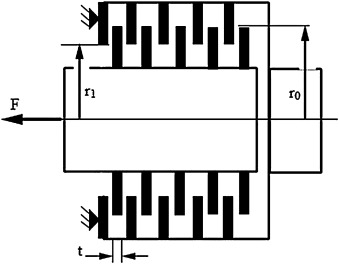
\includegraphics[scale=0.6]{Imgs/MD.jpg}
    \end{center}
    \captionsetup{justification=centering}
    \caption{Schematic view of the multiple disk clutch brake design problem.}\label{fig:MD}
\end{figure}